\chapter[Metodologia]{Metodologia}
\label{cap:metodologia}

Para verificação da conformidade do programa-fonte com as regras sintáticas da linguagem \textit{K}, foi desenvolvido um analisador sintático descendente. Foi construído um projeto para o \textit{parser} com o intuito de facilitar o desenvolvimento e  evitar descoberta de peculiaridades da implementação em uma fase tardia da mesma.

\section{Projeto do analisador sintático}
\label{sec:metodologia_projeto}

Inicialmente, foi realizado um estudo da gramática da linguagem \textit{K}, com o intuito de identificar produções que não possuem características LL(1), isto é, recursão à esquerda e prefixos comuns. Após identificação destas características, as produções que continham as mesmas foram adaptadas para atender aos requisitos de uma gramática LL(1). As alterações realizadas consistiram nos seguintes aspectos:

\begin{itemize}
    \item Adição de um ponto de partida contendo o símbolo inicial original seguido de \$ (fim de arquivo);
    \item Decomposição de regras com recursão à esquerda em duas regras para transformar em recursão à direita;
    \item Adiamento da tomada de decisão em produções com prefixo comum por meio da criação de uma regra específica para o ponto de decisão.
\end{itemize}

A gramática obtida após as adaptações pode ser observada a seguir:

\begin{numberedgrammar}

<program\_prime> ::= <Program> `\$' 

<Program> ::= 'program' <decllist> <stmt-list> 'end' 

<decllist> ::= <decl-list> 
\alt `\lambda' 
    
<decl-list> ::= <decl> <decllist>

<decl> ::= <type> <identifier-list> ;

<identifier-list> ::= <identifier> <possible-ident>

<possible-ident> ::= `,' <identifier> <possible-ident> 
\alt `\lambda' 

<type> ::= <int> 
\alt <string>

<stmt-list> ::= <stmt> <stmtlist>

<stmtlist> ::= <stmt-list> 
\alt `\lambda'

<stmt> ::=   <assign-stmt> ; 
\alt <if-stmt> 
\alt <while-stmt> 
\alt <read-stmt> ';' 
\alt <write-stmt> ';'
	
<assign-stmt> ::= <identifier> '=' <simple-expr>

<if-stmt> ::= 'if' <condition> 'then' <stmt-list> <if-stmt-prime>

<if-stmt-prime> ::=   'end' 
\alt 'else' <stmt-list> <end>
		 
<condition> ::= <expression>

<while-stmt> ::= 'do' <stmt-list> <stmt-sufix>

<stmt-sufix> ::= 'while' <condition> 'end'

<read-stmt> ::= 'scan' '(' <identifier> ')'

<write-stmt> ::= <print> '(' <writable> ')'

<writable> ::= <simple-expr> 
\alt <literal>

<expression> ::= <simple-expr> <expression-prime>

<expression-prime> ::= <relop> <simple-expr> 
\alt `\lambda'

<simple-expr> ::= <term> <simple-expr-prime>

<simple-expr-prime> ::= 	  <addop> <term> <simple-expr-prime> 
\alt `\lambda'

<term> ::= <factor-a> <term-prime>

<term-prime> ::=   <mulop> <factor-a> <term-prime> 
\alt `\lambda'

<factor-a> ::= <factor> 
\alt '!' <factor> 
\alt '-' <factor>

<factor> ::= <identifier> 
\alt <constant> 
\alt '(' <expression> ')'

<relop> ::= '==' 
\alt `>' 
\alt `>=' 
\alt `<' 
\alt `<=' 
\alt `!='

<addop> ::= `+' 
\alt `-' 
\alt `||'

<mulop> ::= `*' 
\alt `/' 
\alt `&&'

\end{numberedgrammar}


Para possibilitar a implementação da metodologia proposta, os \textit{tokens} especificados na gramática da linguagem \textit{K} foram identificados e seus conjuntos \textit{FIRST} e \textit{FOLLOW} foram calculados (Tabela \ref{table:tokens}):

\begin{longtable}{|c | c | c|} 

\hline
 \textbf{Token} & \textbf{Conjunto \textit{FIRST}} & \textbf{Conjunto \textit{FOLLOW}} \\ 
 \hline
 Program & \makecell{program} &  \makecell{\$}\\ 
 \hline
 decllist & \makecell{\lambda, int, string} & \makecell{identifier, do, print, if, scan} \\ 
 \hline
 decl-list & int, string & identifier, do, print, if, scan \\ 
 \hline
 decl & int, string & \makecell{int, string, identifier, do, print, if, scan} \\ 
 \hline
 identifier-list & identifier & ;\\
 \hline
 possible-ident  & ",", \lambda & 	;\\
 \hline
 type  & int, string & identifier \\
 \hline
 stmtlist  & \makecell{\lambda, identifier,\\ do, print, if, scan} & while, end, else\\
 \hline
 assign-stmt & identifier & ;\\
 \hline
 if-stmt & if & \makecell{identifier, do, print, if,\\ scan, while, end, else}\\
 \hline
 if-stmt-prime & end, else & \makecell{identifier, do, print, if,\\ scan, while, end, else}\\
 \hline
 while-stmt & do & \makecell{identifier, do, print, if,\\ scan, while, end, else}\\
 \hline
 stmt-sufix & while & \makecell{identifier, do, print, if,\\ scan, while, end, else}\\
  \hline
 read-stmt & scan & ;\\
  \hline
 write-stmt & print & ;\\
\hline
 writable &	\makecell{literal, !, -, identifier,\\ (, integer-const} & )\\
 \hline
 simple-expr-prime & \lambda, +, -, ||  & \makecell{==, >, >=, <, <=, !=,\\ ), end, then, ;}\\
 \hline
 term-prime &	\lambda, *, /, \&\&  &  \makecell{+, -, ||, ==, >, >=,\\ <, <=, !=, ), end, then, ;}\\
 \hline
 factor-a &	\makecell{!, -, identifier, (,\\ \detokenize{integer_const}, literal} & \makecell{*, /, \&\&, +, -, ||,\\ ==, >, >=, <,\\ <=, !=, ), end, then, ;} \\
 \hline
 factor	& \makecell{identifier, (, \detokenize{integer_const},\\ literal} & \makecell{*, /, \&\&, +, -,\\ ||, ==, >, >=, <,\\ <=, !=, ), end, then, ;} \\
 \hline
 relop	& \makecell{==, >, >=, <,\\ <=, !=} & \makecell{!, -, identifier, (,\\ \detokenize{integer_const}, literal} \\
 \hline
 addop	& \makecell{+, -, ||} & \makecell{!, -, identifier, (,\\ \detokenize{integer_const}, literal} \\
 \hline
 mulop	& \makecell{*, /, \&\&} & \makecell{!, -, identifier, (,\\ \detokenize{integer_const}, literal} \\
 \hline
 constant &	\makecell{\detokenize{integer_const}, literal} & \makecell{*, /, \&\&, +, -,\\ ||, ==, >, >=, <,\\ <=, !=, ), end,\\ then, ;}\\
 \hline
 stmt & \makecell{identifier, do, print,\\ if, scan} & \makecell{identifier, do, print, if,\\ scan, while, end, else}\\
 \hline 
 term &	\makecell{!, -, identifier,\\ (, \detokenize{integer_const}, literal} & \makecell{+, -, ||, ==,\\ >, >=, <, <=, !=,\\ ), end, then, ;}\\
 \hline
 stmt-list	& \makecell{identifier, do, print,\\ if, scan} & while, end, else \\
 \hline
 simple-expr & \makecell{!, -, identifier, (,\\ \detokenize{integer_const}, literal} & \makecell{==, >, >=, <, <=,\\ !=, ), end, then, ;} \\
 \hline
 expression &	\makecell{!, -, identifier, (,\\ integer-const, literal} & \makecell{), end, then}\\
 \hline
 expression-prime &	\makecell{\lambda, ==, >, >=, <, <=, !=} & \makecell{), end, then}\\
 \hline
 
 condition & \makecell{!, -, identifier, (,\\ integer\_const, literal} & \makecell{end, then}\\
 \hline
 
\caption{Produções e seus conjuntos \textit{first} e \textit{follow}.}
\label{table:tokens}
\end{longtable}

Após o cálculo dos conjuntos \textit{first} e follow dos símbolos não-terminais, os mesmos (juntamente com a gramática modificada) foram utilizados para construir a tabela do \textit{parser}. É possível observar que a tabela não possui entradas duplicadas. Portanto, é possível implementar um \textit{parser} recursivo descendente para a mesma. A tabela do \textit{parser} foi movida para a próxima página para facilitar sua visualização.

\afterpage{
    \clearpage
    \thispagestyle{empty}% empty page style (?)
    \begin{landscape}% Landscape page
    \fontsize{10}{10}\selectfont
    \begin{adjustwidth}{-2cm}{}

        \centering % Center table
        \begin{tabular}{|c | c | c| c | c | c | c | c | c |c | c | c| c | c | c | c | c | c | c |}
          \hline
 \textbf{Produção} & \textbf{\$} & \textbf{program} & \textbf{end} & \textbf{identifier} & \textbf{,} & \textbf{int} & \textbf{string} & \textbf{;} & \textbf{=} & \textbf{if} & \textbf{then} & \textbf{else} & \textbf{do} & \textbf{while} & \textbf{scan} & \textbf{(} & \textbf{)} & \textbf{print} \\ 
 \hline
 Program & & 2 & & & &  & & & & & & & & & & & &\\ 
 \hline
 decllist & & & & 3 &  &  & & &  & 4 & &  & 4 &  & 4 & & & 4\\ 
 \hline
 decl-list & & & & 5 &  &  & & &  &  & &  &  &  &  & & & \\ 
 \hline
  decl & & & & 6 &  &  & & &  &  & &  &  &  &  & & & \\ 
   \hline
  identifier-list & & & & 7 &  &  & & &  &  & &  &  &  &  & & & \\ 
 \hline
possible-ident & & & &  & 8 &  & & &  & 8 &  &  & 8 & & 8 & & & 9 \\ 
 \hline
 type & & & &  &  & 10 & 11 & &  &  &  &  &  & & 8 & & &  \\ 
 \hline
  stmtlist & & & 14 & 13 &  &  &  & &  & 13 &  & 14 & 12 & 14 & 13 & & & 13  \\ 
 \hline
   stmt-list & & &  & 12 &  &  &  & &  & 12 &  &  & 12 &  & 12 & & & 12  \\ 
 \hline
 
  stmt & & &  & 15 &  &  &  & &  & 16 &  &  & 17 &  & 18 & & & 19  \\ 
 \hline
  assign-stmt & & &  & 20 &  &  &  & &  &  &  &  &  &  &  & & &   \\ 
 \hline
  assign-stmt & & &  & 20 &  &  &  & &  &  &  &  &  &  &  & & &   \\ 
 \hline
  if-stmt & & &  &  &  &  &  & &  & 21 &  &  &  &  &  & & &   \\ 
 \hline 
  if-stmt-prime & & & 22 &  &  &  &  & &  &  &  & 23 &  &  &  & & &   \\ 
 \hline
  condition & & & & 24 & & & & & & & & & & & & 24 & &   \\ 
 \hline
 while-stmt & & & & & & & & & & & & & 25 & & & & &   \\ 
 \hline
 stmt-sufix & & & & & & & & & & & & & & 26 & & & &   \\ 
\hline
 read-stmt & & & & & & & & & & & & & & & 27 & & &   \\ 
\hline
 write-stmt & & & & & & & & & & & & & & & & & & 28  \\ 
\hline
 write-stmt & & & & & & & & & & & & & & & & & & 28  \\ 
\hline
 writable & & & & 29 & & & & & & & & & & & & 29 & &  \\
 \hline
 expression & & & & 31 & & & & & & & & & & & & 31 & &  \\
 \hline
 expression-prime & & & 33 & & & & & & & & 32 & & & & & & 32 & \\
 \hline
 simple-expr & & & & 34 & & & & & & & & & & & & 34 & & \\
 \hline
 simple-expr-prime & & & 36 &  & & & & & & & 36 & & & & & 34 & 36 & \\
 \hline
 term & & &  & 37 & & & & & & &  & & & & & 37 &  & \\
 \hline
 term-prime & & & 39 & & & & & & & & 39 & & & & & & 39 & \\
 \hline
 factor-a & & & & 40 & & & & & & & & & & & & 40 & & \\
 \hline
 factor & & & & 43 & & & & & & & & & & & & 45 & & \\
 
 \hline\\
        \end{tabular}
        \captionof{table}{Primeira parte da tabela do parser LL(1)}% Add 'table' caption
    \end{adjustwidth}{}{}
    \end{landscape}
    \clearpage% Flush page
}




\afterpage{
    \clearpage
    \thispagestyle{empty}% empty page style (?)
    \begin{landscape}% Landscape page
    \fontsize{10}{10}\selectfont
    \begin{adjustwidth}{-2cm}{}
        \centering % Center table

        \begin{tabular}{|c | c | c| c | c | c | c | c | c |c | c | c| c | c | c | c |}
          \hline
 \textbf{literal} & \textbf{!} & \textbf{-} & \textbf{==} & \textbf{>} & \textbf{>=} & \textbf{<} & \textbf{<=} & \textbf{!=} & \textbf{+} & \textbf{||} & \textbf{*} & \textbf{/} & \makecell{\textbf{\&\&}} & \textbf{integer-const} & \textbf{literal} \\ 
 \hline
  condition & 24 & 24 & & & & & & & & & & & & 24 & 24\\ 
 \hline
 while-stmt & & & & & & & & & & & & & & & \\
 \hline
 stmt-sufix & & & & & & & & & & & & & & &    \\ 
\hline
 read-stmt & & & & & & & & & & & & & & &   \\ 
\hline
 write-stmt & & & & & & & & & & & & & & &  \\ 
\hline
 write-stmt & & & & & & & & & & & & & & &   \\ 
\hline
 writable & 29 & 29 & & & & & & & & & & & & 29 & 30  \\
\hline
 expression & 31 & 31 & & & & & & & & & & & & 31 & 31  \\
 \hline
 expression-prime & & & 32 & 32 & 32 & 32 & 32 & 32 & & & & & & &  \\
 \hline
simple-expr & 34 & 34 & & & & & & & & & & & & 34 & 34  \\
\hline
simple-expr-prime & & 35 & 36 & 36 & 36 & 36 & 36 & 36 & 35 & 35 & & & & &   \\
 \hline
term & 37 & 37 &  &  &  & & & & & & & & & 37 & 37  \\
 \hline
term &  & 39 & 39 & 39 & 39 & 39 & 39 & 39 & 39 & 39 & 38 & 38 & 38 &  &   \\
\hline
factor-a & 41 & 42 & & & & & & & & & & & & 40 & 40  \\
\hline
factor &  &  & & & & & & & & & & & & 44 & 44  \\
\hline
relop & & & 46 & 47 & 48 & 49 & 50 & 51 & & & & & & 44 & 44  \\
\hline
addop & & 53 & & & & & & & 52 & 54 & & & & &   \\
\hline
mulop & & & & & & & & & & & 55 & 56 & 57 & & \\
\hline


 \hline  \\
        \end{tabular}
        \captionof{table}{Segunda parte da tabela do parser LL(1)}% Add 'table' caption
    \end{adjustwidth}{}{}
    \end{landscape}
    \clearpage% Flush page
}




\newpage
\section{Implementação do analisador sintático}

A linguagem de programação Java foi escolhida para a implementação do analisador sintático do compilador em continuação a implementação prévia do primeiro trabalho prático e devido aos recursos de processamento de texto e estruturas de dados disponíveis na linguagem, além de sua compilação híbrida que permite execução multiplataforma.

\subsection{Arquitetura da implementação}

  O diagrama de classe gerado no trabalho anterior(Figura \ref{fig:diagram}) foi atualizado para compreender as alterações e avanços realizados no projeto. A arquitetura do KPiler baseou-se nas diretrizes e recomendações de \cite{andrew2002modern}.

\begin{figure}[!h]
\centering
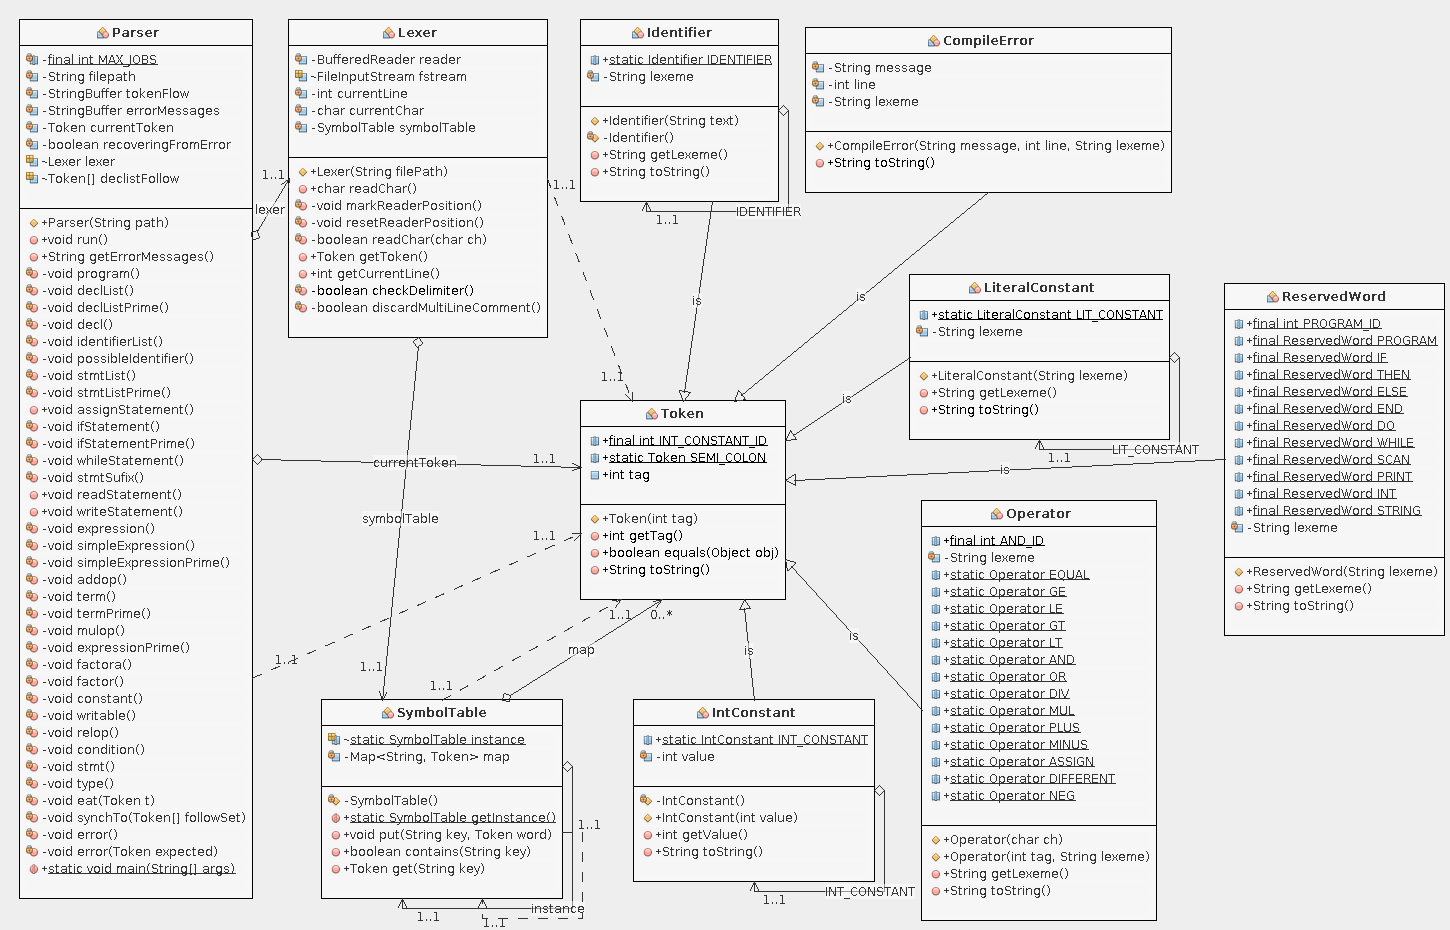
\includegraphics[width=16cm,height=20cm,keepaspectratio]{img/class_diagram.png}
\caption{Diagrama de classe do compilador, as classes utilitárias foram omitidas para facilitar o entendimento.}
\label{fig:diagram}
\end{figure}

Nesta etapa do projeto, somente as classes \textit{Token}, \textit{Lexer} e \textit{Parser} foram alteradas significativamente. Estas classes e funções estão detalhados a seguir:

\begin{itemize}
    \item \textbf{Parser (analisador sintático):} classe que contem o ponto de entrada (método \textit{main}) do programa. Uma requisição é feita à classe Lexer para obter o fluxo de \textit{tokens}, de modo à implementar compilação em um passo. A classe possui implementação multi-thread possibilitando processamento de vários arquivos simultaneamente. Para cada símbolo não-terminal da gramática foi implementado um método contendo as respectivas cláusulas da gramática. Os métodos \textit{error()}, \textit{synchTo(Token[] followSet)} e a \textbf{flag} booleana \textbf{recoveringFromError} foram utilizadas na implementação de erro em modo pânico.
    
    \item \textbf{Lexer (analisador léxico):} lê o programa fonte caractere a caractere, buscando sequências de caracteres significativas (lexemas) que casem com o padrão de algum \textit{token}. Possui estruturas para leitura do arquivo, armazenamento da linha corrente e um ponteiro para a tabela de símbolos. O método \textit{getToken()} contem a implementação dos autômatos para reconhecimento de \textit{tokens}. Nesta etapa do projeto, a mesma foi alterada para detectar símbolos não aceitos pela linguagem. Essa decisão foi movida pelo intuito de simplificar a implementação do analisador sintático delegando a responsabilidade de reconhecimento de símbolos não aceitos ao analisador léxico.
    
    \item \textbf{Token:} contem o dicionário de \textit{tags} e um atributo inteiro para armazenamento do mesmo. É classe pai das classes \textit{CompileError}, \textit{Identifier},\textit{IntConstant}, \textit{LiteralConstant}, \textit{ReservedWord} e \textit{Operator}. Estas classes implementam polimorfismo no método \textit{toString()} para exibir os \textit{tokens} em seu formato apropriado. Foi incorporado o método \textit{equal(Token t)} à classe \textit{Token} nesta etapa do trabalho para facilitar as comparações de igualdade.
    
\end{itemize}

\subsection{Recuperação de erro}

Com o intuito de exibir a maior quantidade de erros possível ao usuário, recuperação de erro em modo pânico foi implementada. Após ocorrência de um erro, \textit{tokens} são consumidos até que se encontre um \textit{token} de um conjunto especificado. Utilizou-se o conjunto \textit{follow} de cada não-terminal como heurística para recuperação de erro.

Com este recurso, foi possível exibir maior quantidade de erros em uma única compilação ao usuário. Os resultados da implementação podem ser observados no Capítulo \ref{cap:avaliacao} (Avaliação dos resultados).

\subsection{Recursos adicionais}

O compilador foi construído em uma arquitetura paralela, que permite que vários arquivos sejam analisados paralelamente pelos analisadores léxico e sintático. Para cada arquivo, são criados um objeto da classe \textit{Lexer} e um objeto da classe \textit{Parser} preservando a estrutura de compilação em um passo solicitada pela orientadora.